\chapter{Resultados} \label{chap:resultados} % ### 7.

Neste capítulos serão apresentados os resultados obtidos com a \hyperref[sec:sistema]{implementação do sistema} de gerenciamento de suporte à decisão discutido ao longo deste trabalho. Serão apresentadas as \hyperref[ssec:paginas]{páginas} desenvolvidas, bem como as \hyperref[ssec:funcionalidades]{funcionalidades} implementadas.

% \section{UENF}

% \section{Entrevistas}

% \section{Formulário}

\section{Sistema desenvolvido} \label{sec:sistema}

O sistema foi desenvolvido utilizando a linguagem de programação JavaScript em conjunto com o React, um framework de desenvolvimento de interfaces de usuário. O sistema consiste de um conjunto de \hyperref[ssec:paginas]{oito páginas} principais, das quais emergem diversas \hyperref[ssec:funcionalidades]{funcionalidades}.

\subsection{Páginas} \label{ssec:paginas}

A página inicial (\autoref{fig:main}) apresenta um resumo do objetivo e seu funcionamento básico, informa também sobre atalhos possíveis para uso mais dinâmico do sistema.
básica de dados, se mostra como uma página importante para futuros desenvolvimentos no campo de alocação de alunos em turmas.

\begin{MyCenteredFigure} \caption{Página inicial do sistema} \label{fig:main}
  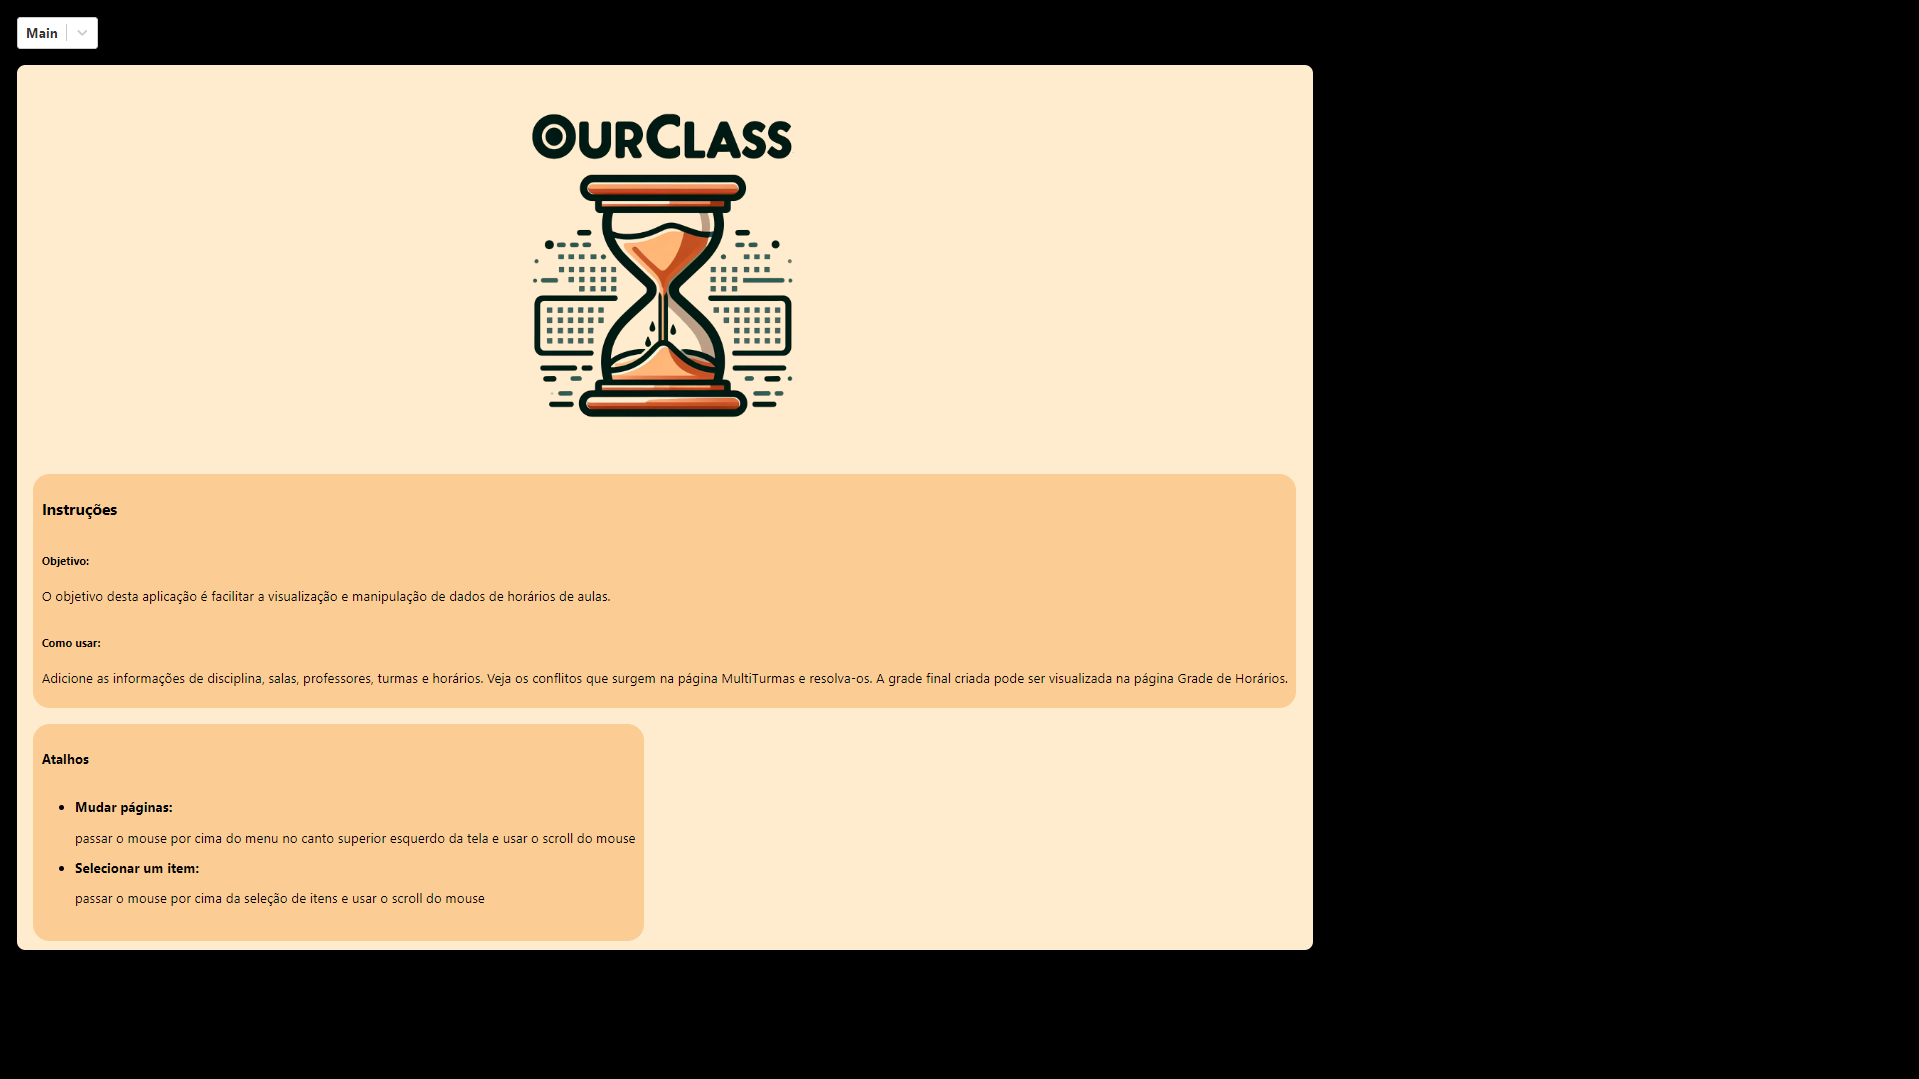
\includegraphics[width=\textwidth]{files/img/2.02!7-resultados/1-Main.png}
\end{MyCenteredFigure}

A página \textbf{MultiTurmas} é repartida em três partes principais: a primeira, com filtros para a seleção das turmas mostradas (\autoref{fig:multiFiltros}); a segunda, com a visualização dos conflitos de horários entre as turmas selecionadas (\autoref{fig:multiConflitos}); e a terceira, com a visualização das disciplinas pendentes de alocação nas turmas selecionadas (\autoref{fig:multiDisciplinas}).

\begin{MyCenteredFigure} \caption{Página de multiturmas com filtros} \label{fig:multiFiltros}
  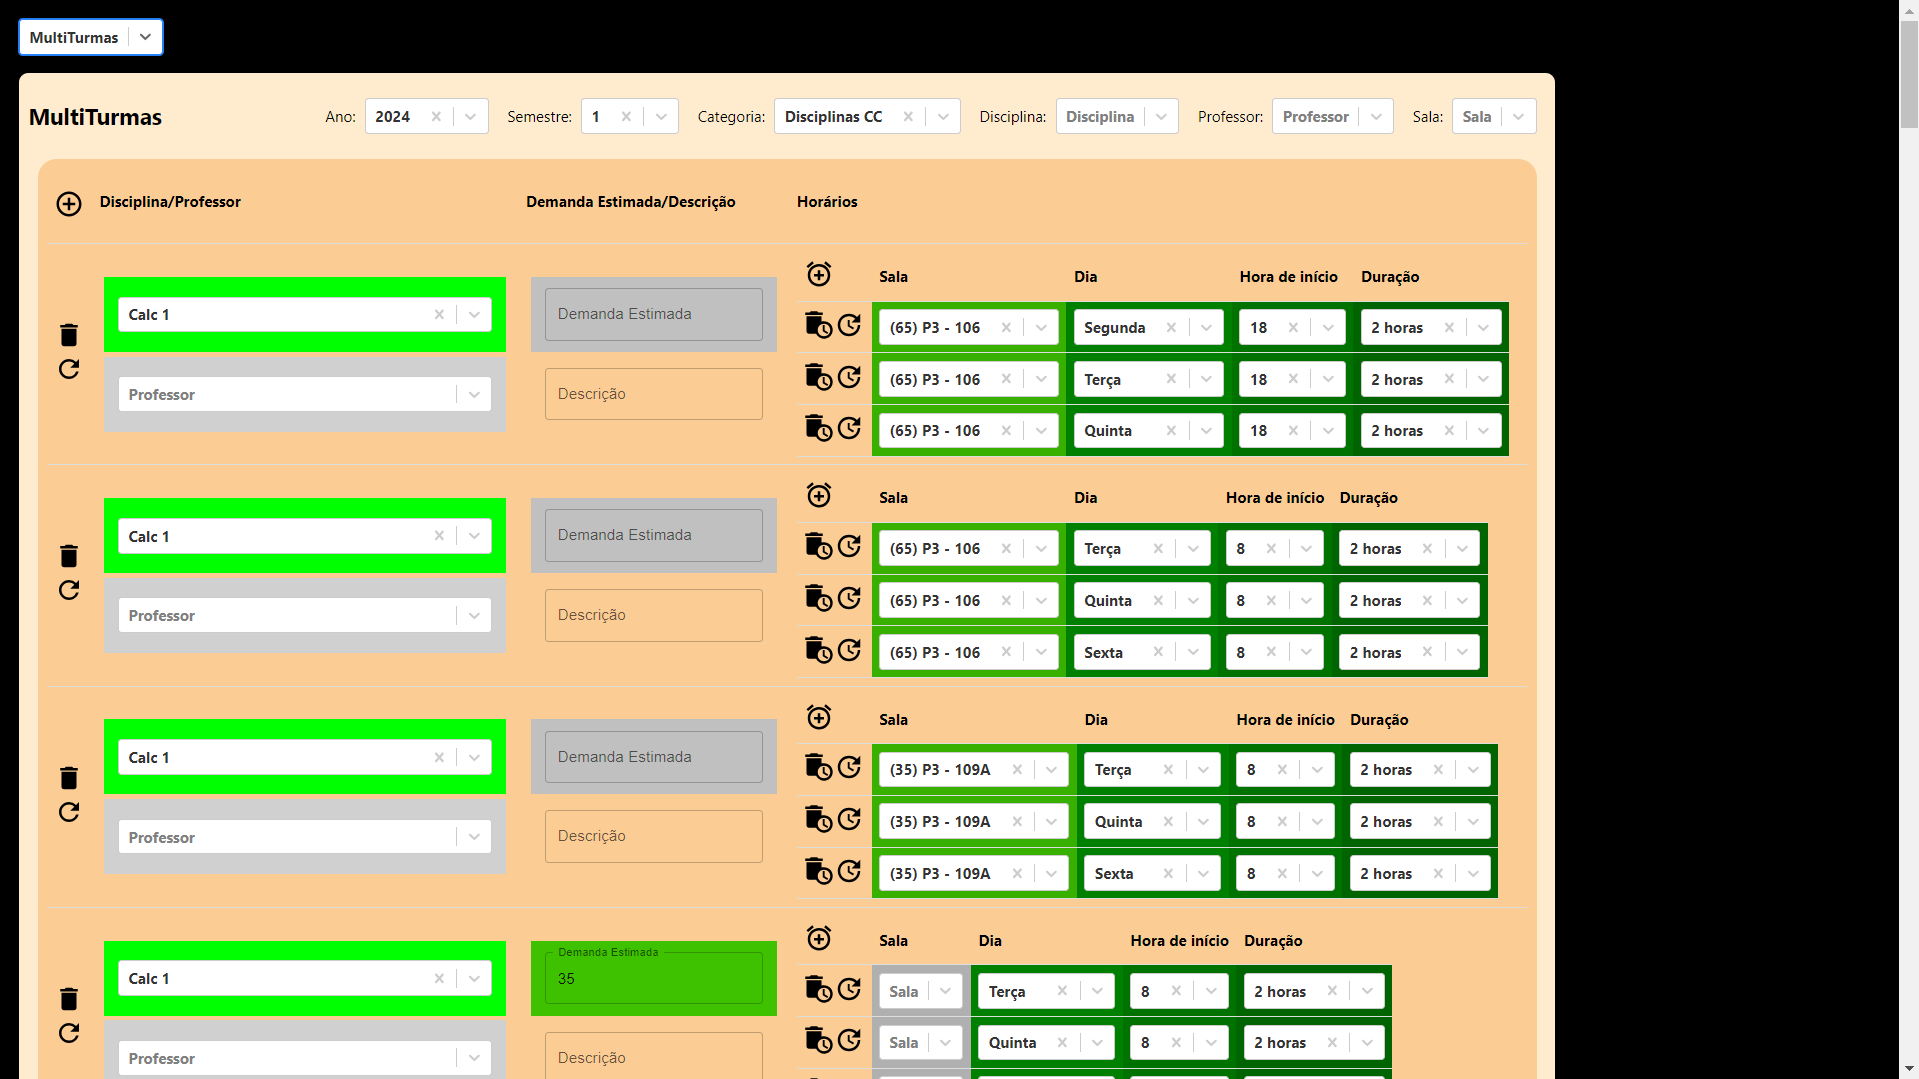
\includegraphics[width=\textwidth]{files/img/2.02!7-resultados/2-Multiturmas-Filtros.png}
\end{MyCenteredFigure}

\begin{MyCenteredFigure} \caption{Página de multiturmas com conflitos} \label{fig:multiConflitos}
  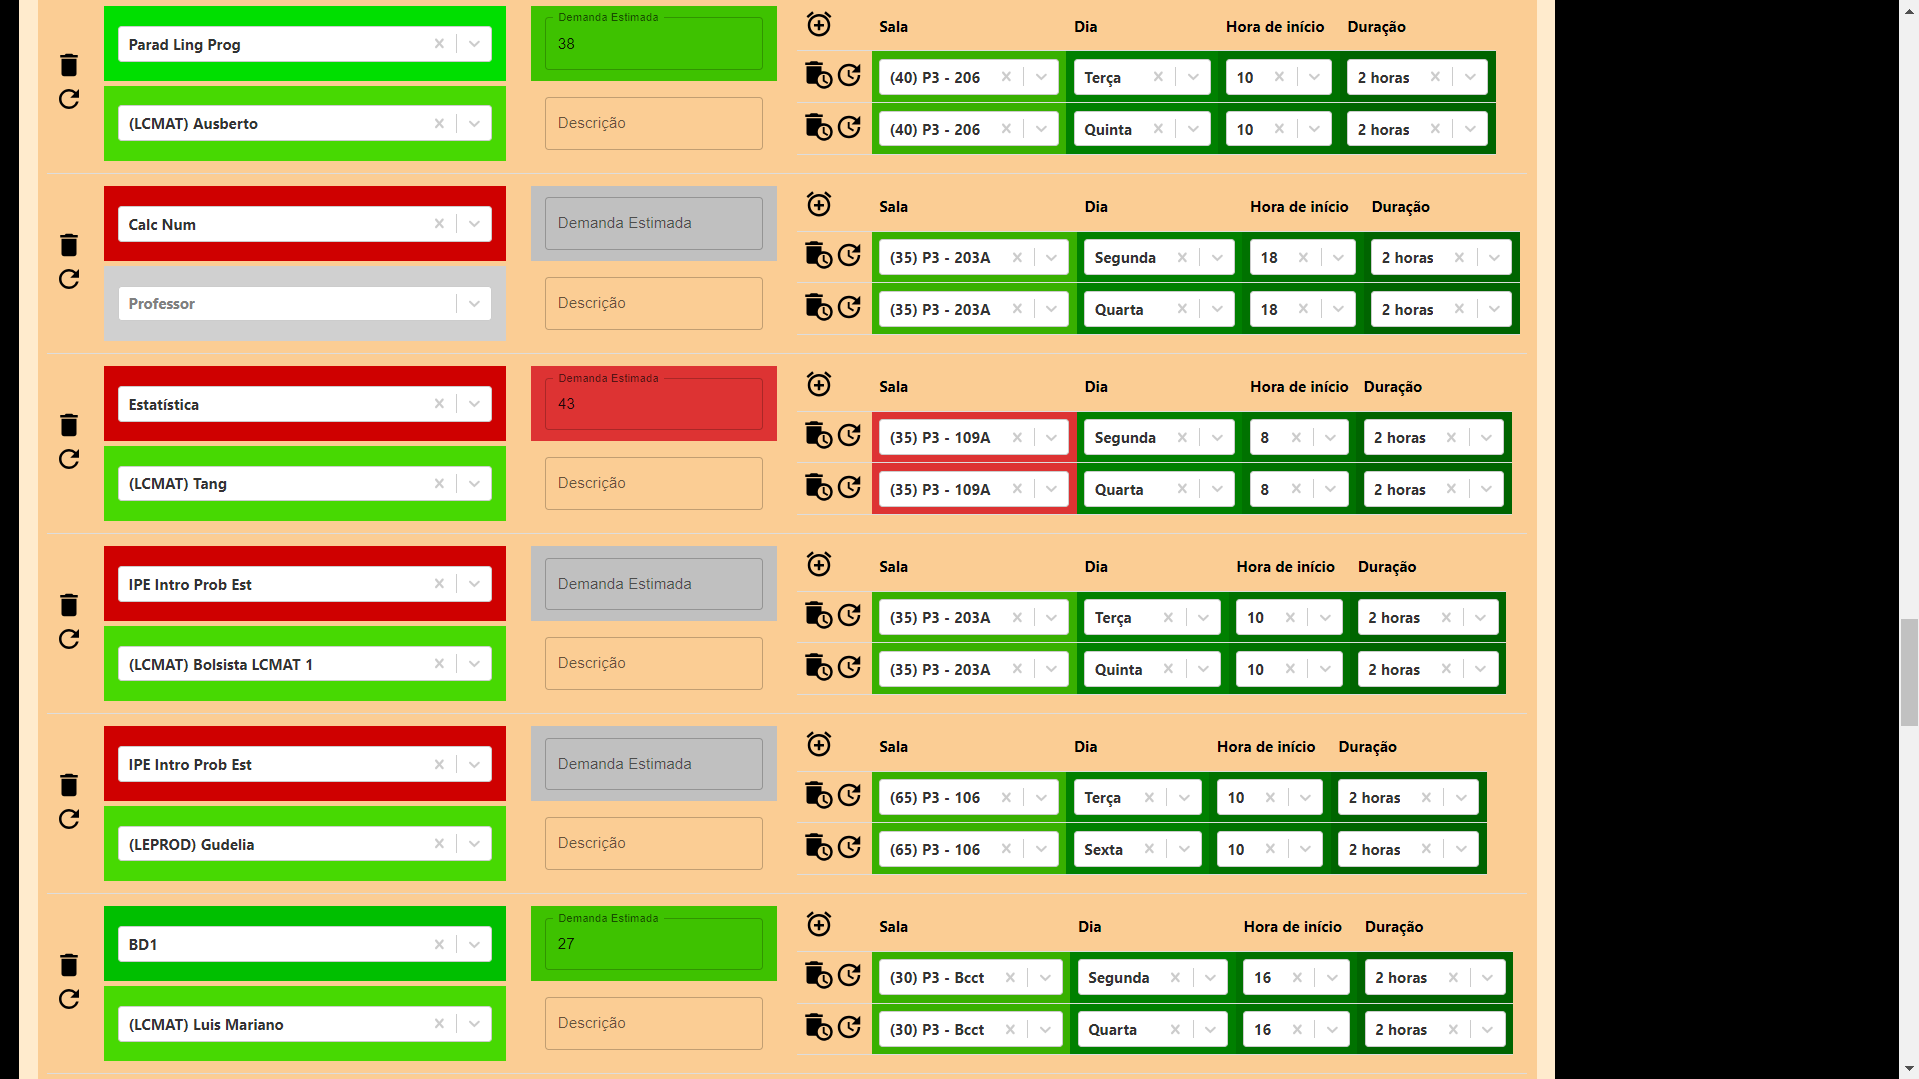
\includegraphics[width=\textwidth]{files/img/2.02!7-resultados/3-Multiturmas-Conflitos.png}
\end{MyCenteredFigure}

\begin{MyCenteredFigure} \caption{Página de multiturmas com disciplinas pendentes} \label{fig:multiDisciplinas}
  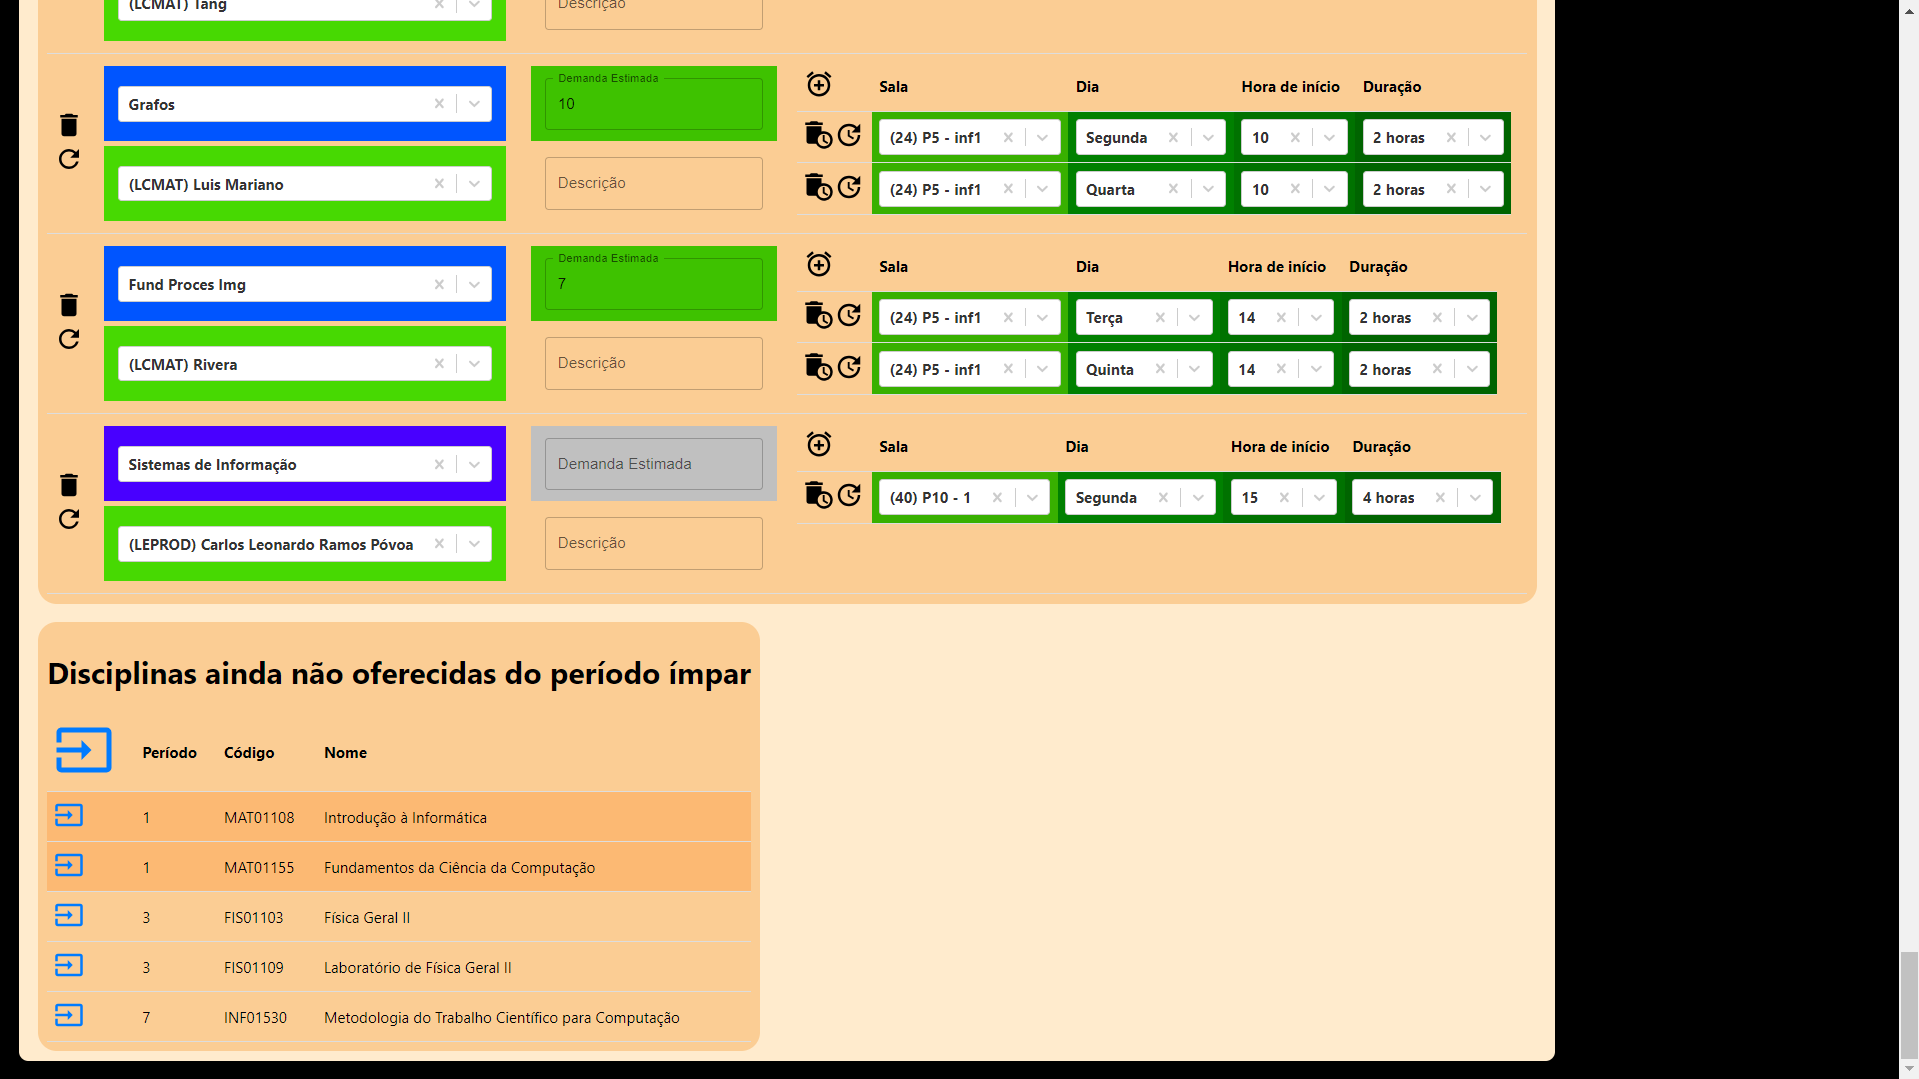
\includegraphics[width=\textwidth]{files/img/2.02!7-resultados/4-Multiturmas-DisciplinasPendentes.png}
\end{MyCenteredFigure}

A página \textbf{Grade de Horários} (\autoref{fig:grade}) apresenta a grade de horários de todas as turmas, podendo também haver a filtragem de quais turmas serão mostradas.

\begin{MyCenteredFigure} \caption{Página de grade de horários} \label{fig:grade}
  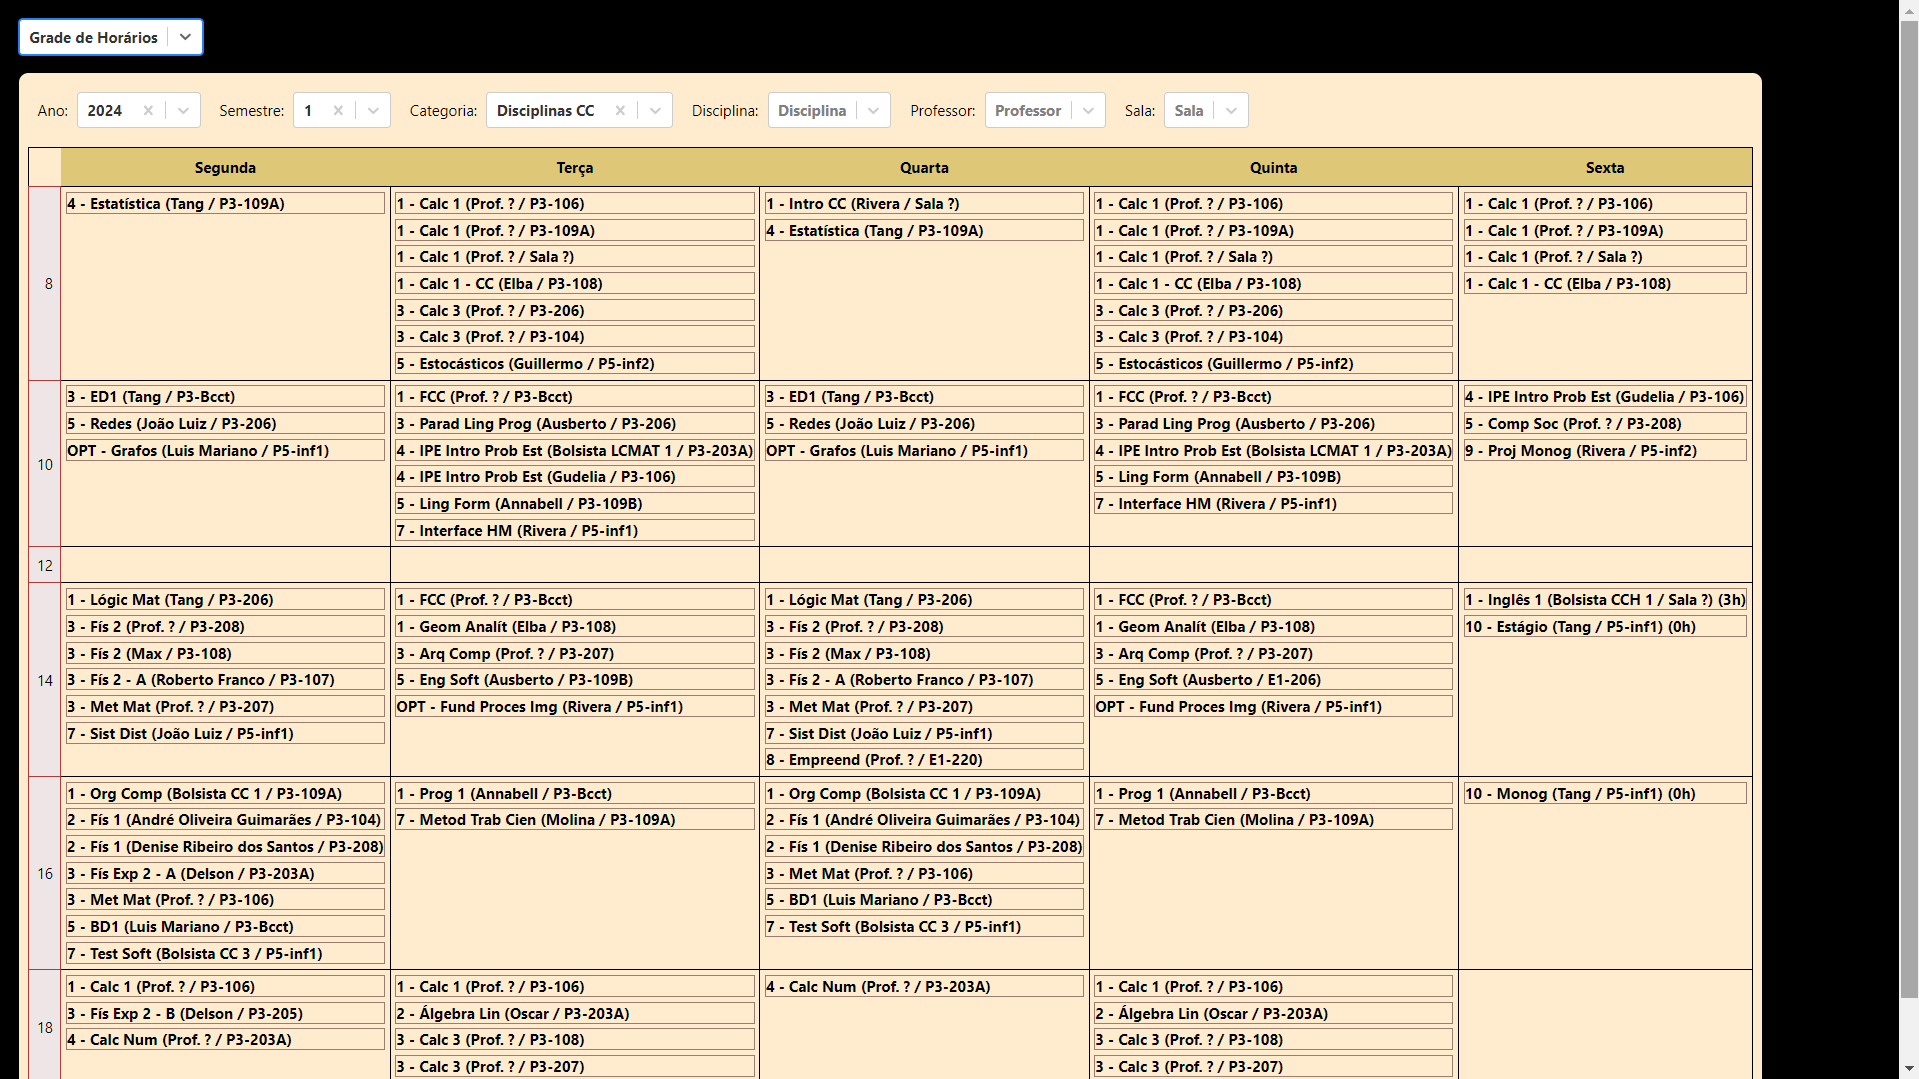
\includegraphics[width=\textwidth]{files/img/2.02!7-resultados/5-Grade de Horários.png}
\end{MyCenteredFigure}

A página \textbf{Turmas} (\autoref{fig:turmas}) apresenta todas as turmas cadastradas, podendo ser feita a edição ou exclusão individual de cada uma delas. Embora ela apresente um funcionamento similar à página MultiTurmas, tem potencial para trabalhar posteriormente com um ajuste fino específico de cada turma.

\begin{MyCenteredFigure} \caption{Página de turmas} \label{fig:turmas}
  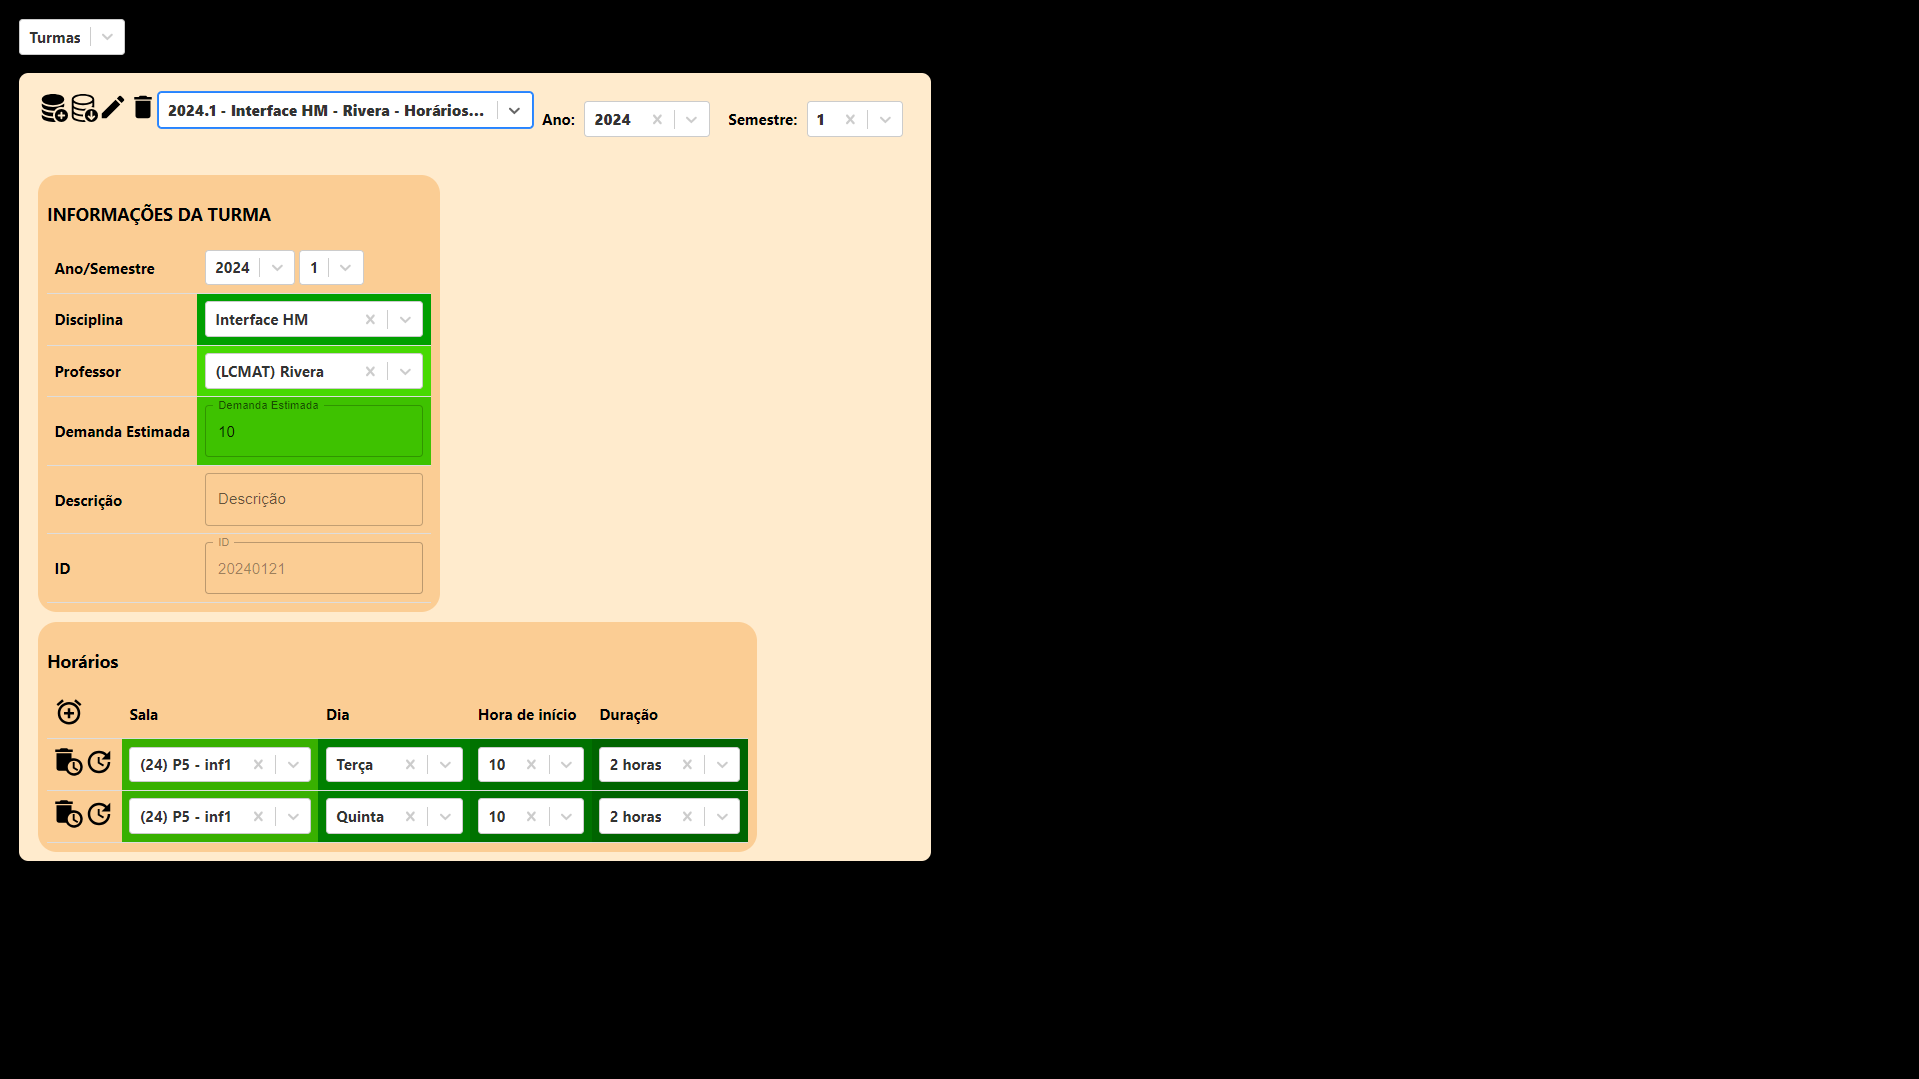
\includegraphics[width=\textwidth]{files/img/2.02!7-resultados/6-Turmas.png}
\end{MyCenteredFigure}

As páginas \textbf{Professores} (\autoref{fig:professores}), \textbf{Salas} (\autoref{fig:salas}) e \textbf{Disciplinas} (\autoref{fig:disciplinas}) apresentam um funcionamento muito similar entre si. Todas elas permitem as operações de criação, leitura, atualização e exclusão de seus respectivos itens. Além de apresentar também uma tabela inferior onde são listadas os horários histórias em que cada um desses itens foi alocado, podendo haver também a filtragem por ano, semestre, dia e hora.

\begin{MyCenteredFigure} \caption{Página de professores} \label{fig:professores}
  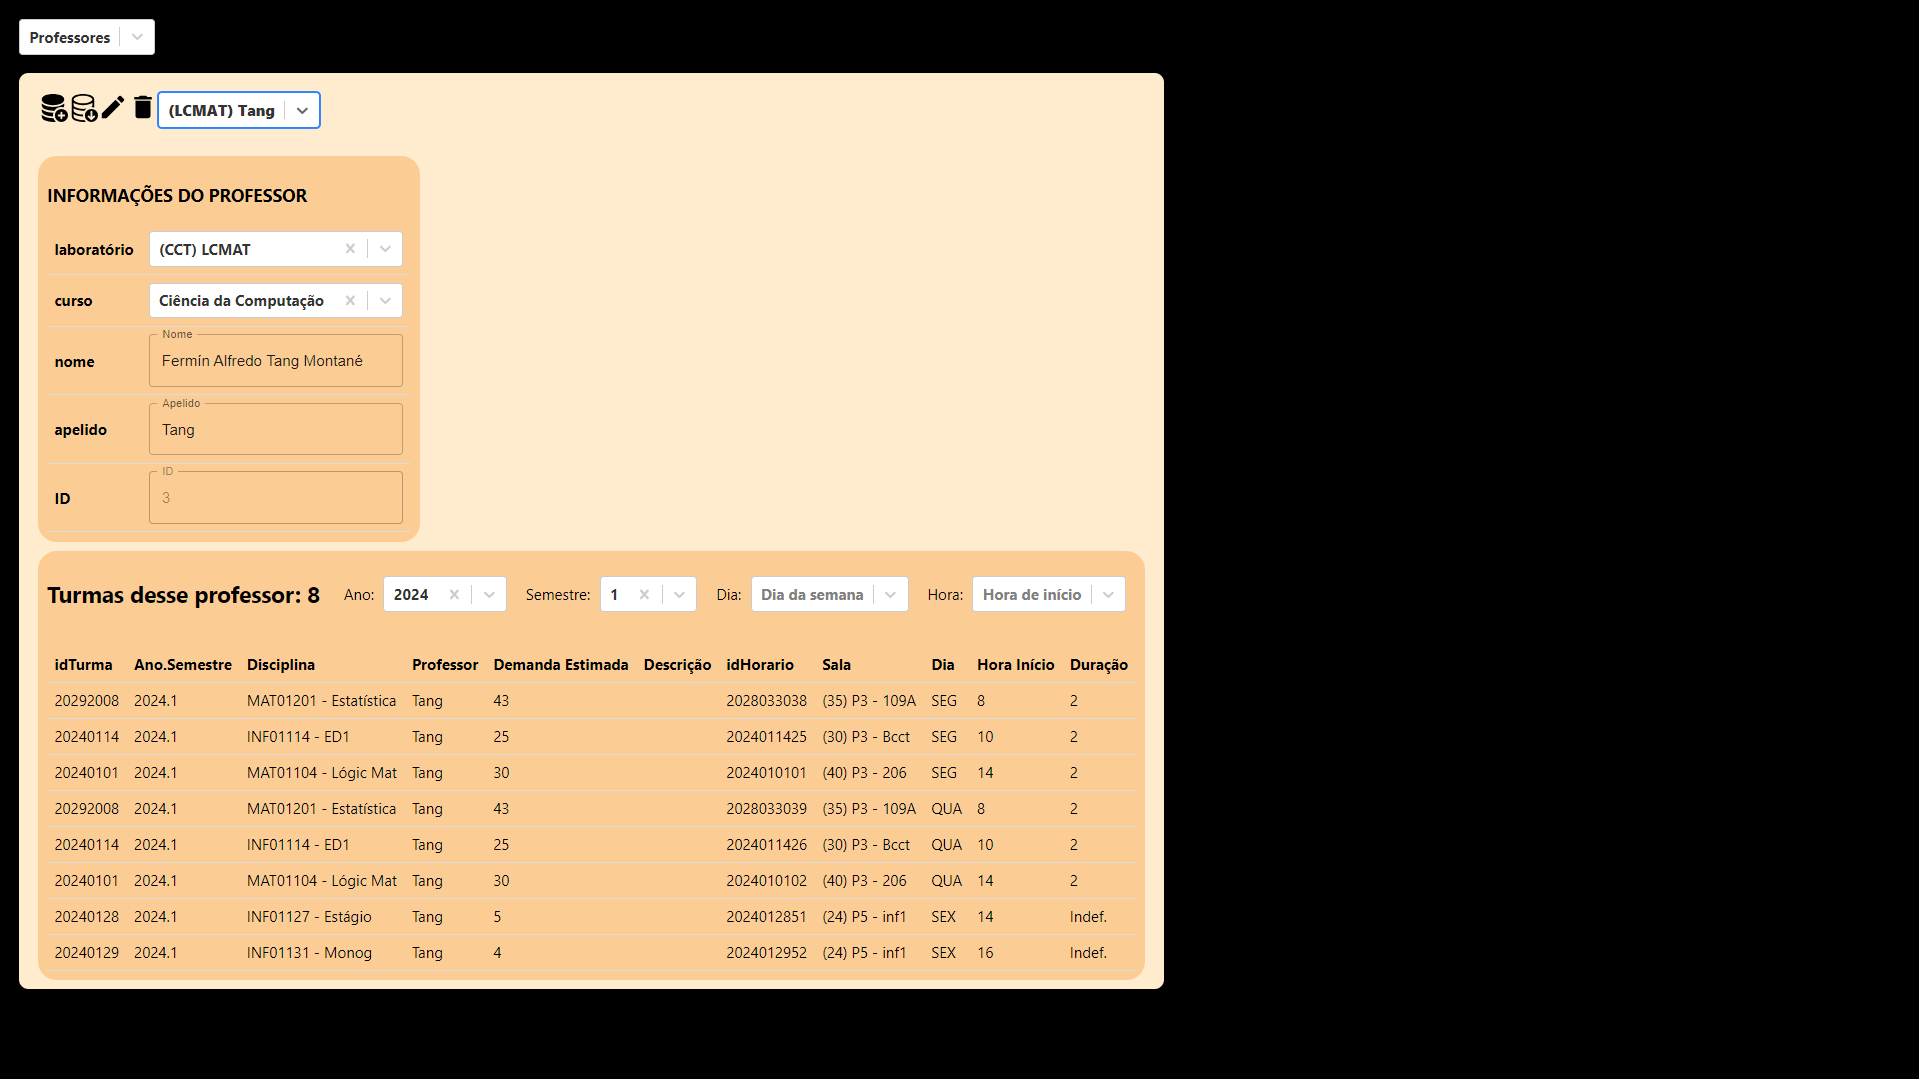
\includegraphics[width=\textwidth]{files/img/2.02!7-resultados/7-Professores.png}
\end{MyCenteredFigure}

\begin{MyCenteredFigure} \caption{Página de salas} \label{fig:salas}
  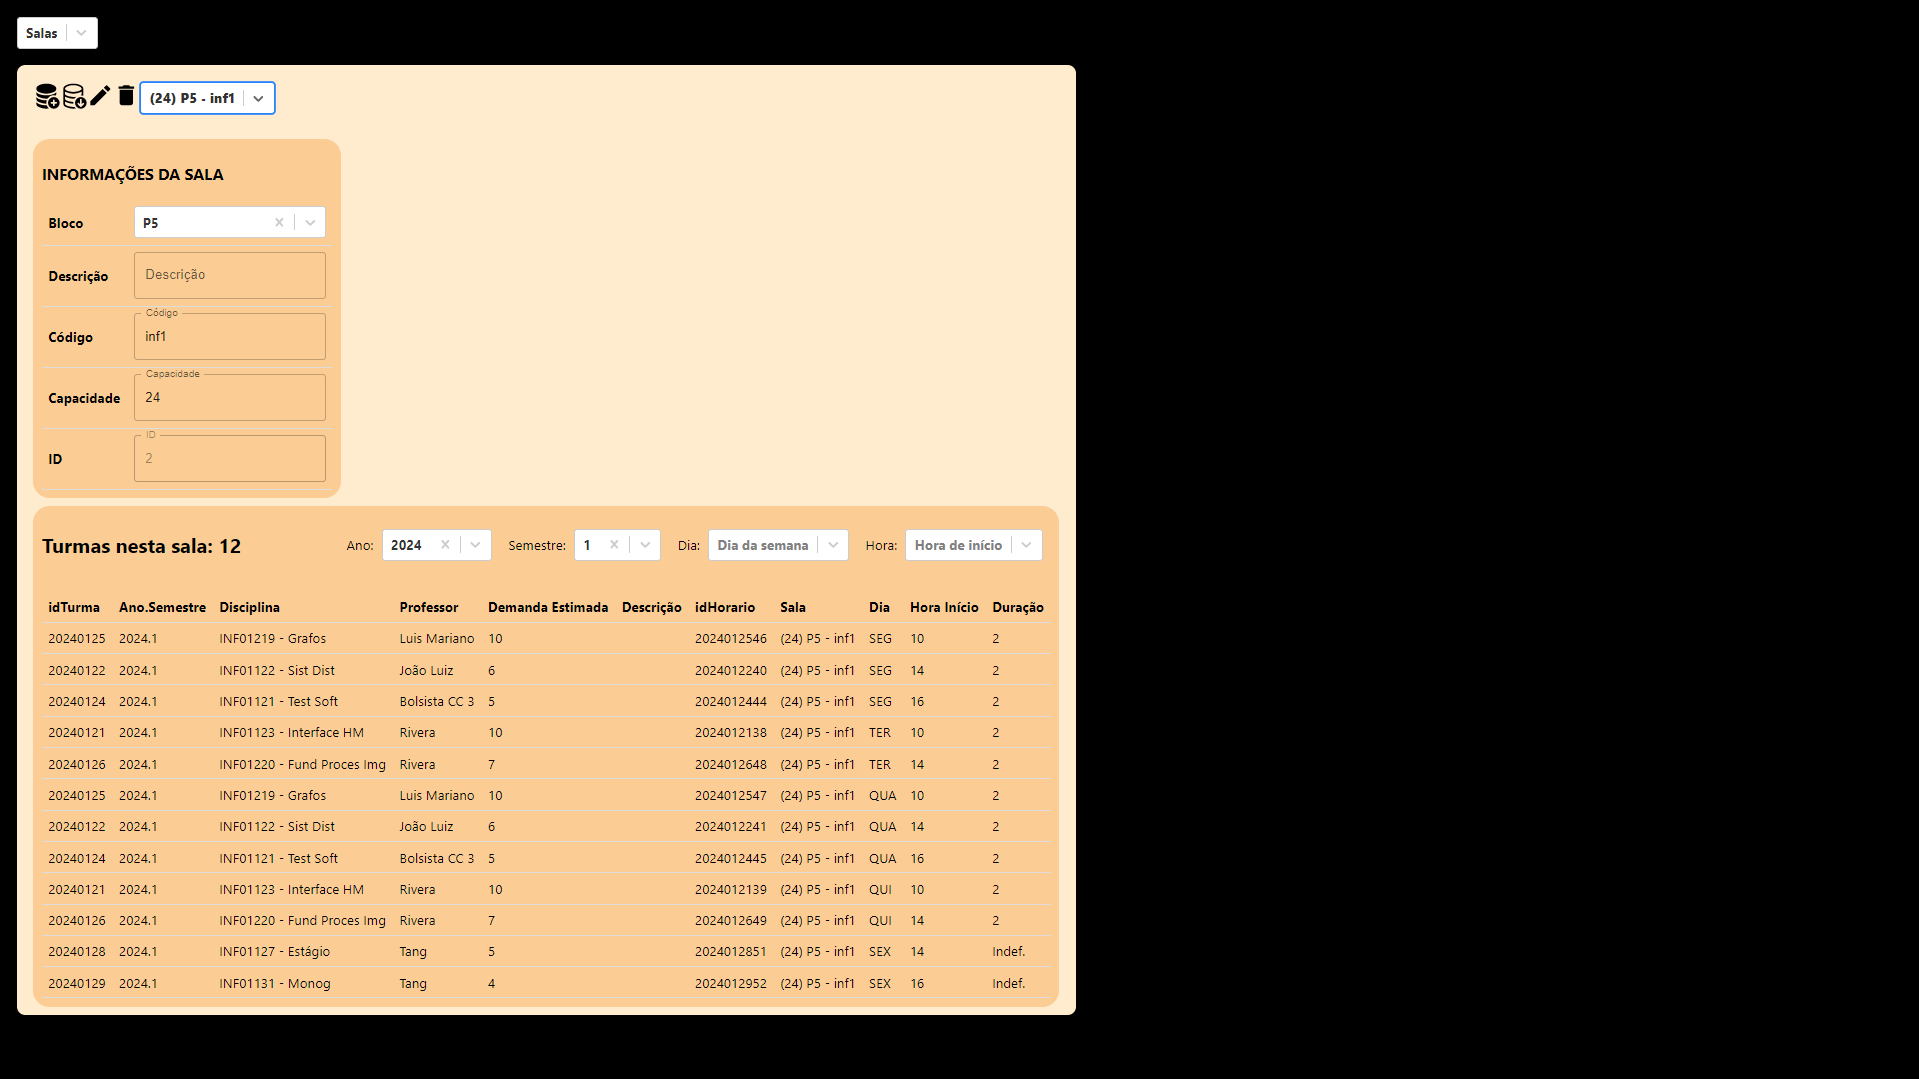
\includegraphics[width=\textwidth]{files/img/2.02!7-resultados/8-Salas.png}
\end{MyCenteredFigure}

\begin{MyCenteredFigure} \caption{Página de disciplinas} \label{fig:disciplinas}
  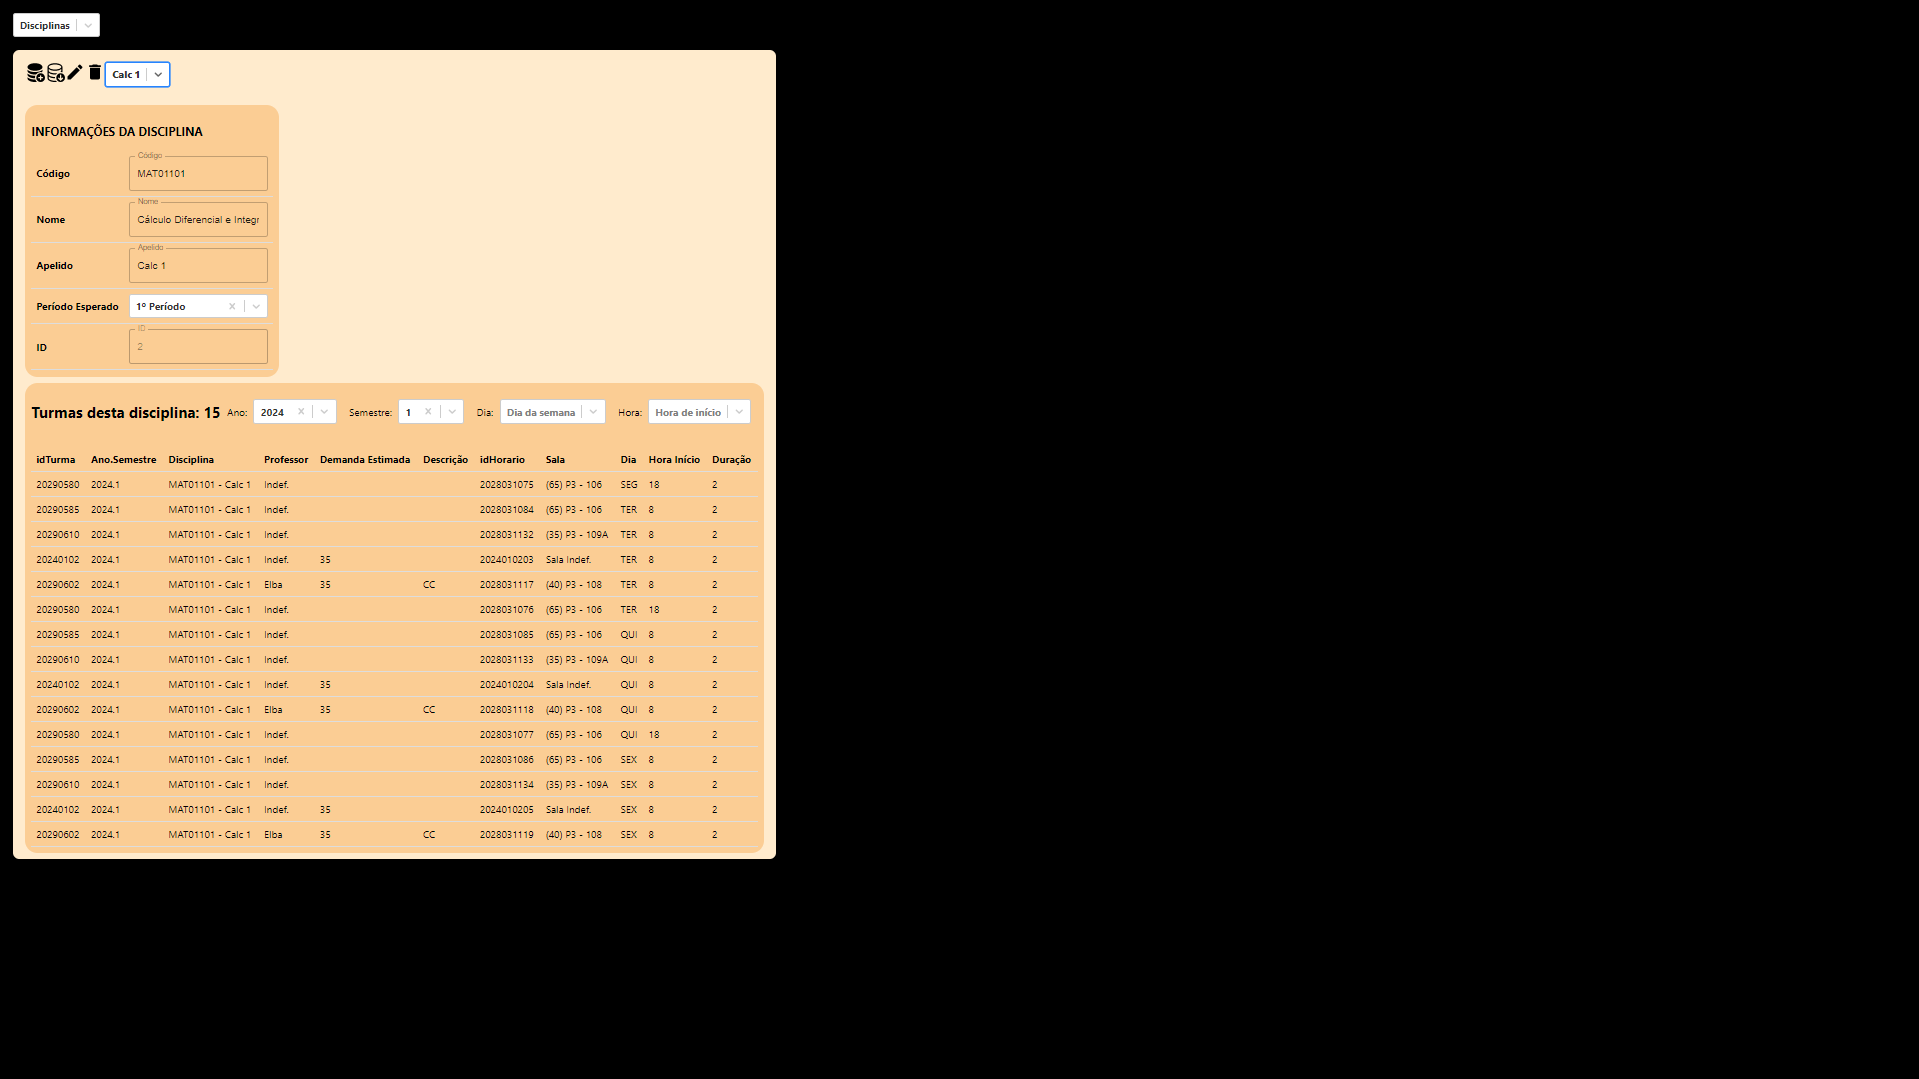
\includegraphics[width=\textwidth]{files/img/2.02!7-resultados/9-Disciplinas.png}
\end{MyCenteredFigure}

A página \textbf{Alunos} (\autoref{fig:alunos}), por fim, apresenta a possibilidade de visualização de todos os alunos cadastrados. Mesmo não possuindo funcionalidades além da manipulação 

\begin{MyCenteredFigure} \caption{Página de alunos} \label{fig:alunos}
  
\includegraphics[width=\textwidth]{files/img/2.02!7-resultados/10-Aluno.png}
\end{MyCenteredFigure}

\subsection{Funcionalidades} \label{ssec:funcionalidades}

Nas páginas apresentadas, foram implementadas diversas funcionalidades que permitem a interação do usuário com o sistema. Dentre elas, destacam-se as \hyperref[sssec:CRUD]{quatro operações básicas de armazenamento persistente}, a \hyperref[sssec:Análise histórica]{análise histórica}, a \hyperref[sssec:Criação de grade inicial]{criação de grade inicial}, a \hyperref[sssec:Visualização de conflitos]{Visualização de conflitos} e a \hyperref[sssec:Visualização de tabelas horárias]{visualização das tabelas horárias}.

\subsubsection{CRUD} \label{sssec:CRUD}

Com exceção da página inicial e da página de grade de horários, todas as páginas apresentam as operações de criação, leitura, atualização e exclusão de seus respectivos itens. Isso se dá pois esta é a função básica de um sistema de gerenciamento de banco de dados, sendo necessária para que todas as outras funcionalidades possam ser implementadas e utilizáveis.

\subsubsection{Análise histórica} \label{sssec:Análise histórica}

O conceito da \textbf{Análise Histórica} é a capacidade de visualizar quais foram todos os horários em que um determinado item foi alocado. Isso é útil para avaliar os padrões emergentes nas alocações dos recursos.

\subsubsection{Criação de grade inicial} \label{sssec:Criação de grade inicial}

A \textbf{Criação de Grade Inicial}, já descritas no \hyperref[ssec:Heurística]{segmento sobre heurística de criação de grade}, é uma funcionalidade que permite a criação de uma grade de horários inicial através da avaliação das alocações anteriores para determinada disciplina. Através dela é possível criar uma grade de horários inicial para o curso de Ciência da Computação em poucos segundos.

\subsubsection{Visualização de conflitos} \label{sssec:Visualização de conflitos}

Na página \textbf{Turmas} e principalmente na página \textbf{MultiTurmas}, é possível visualizar os conflitos existentes entre as turmas. Os \hyperref[sec:conflitos]{conflitos} são apresentados de forma clara e objetiva, permitindo a rápida identificação e posterior resolução.

\subsubsection{Visualização de tabelas horárias} \label{sssec:Visualização de tabelas horárias}

Por fim, especificamente na página \textbf{Grade de Horários}, é possível visualizar as tabelas horárias de todas as turmas cadastradas, podendo haver também a filtragem por ano, semestre, categoria, disciplina, professor e sala. Com esta visualização tabular, pode-se gerar as grades de horários específicas das turmas de disciplinas de cada um dos períodos letivos, bem como distingue as turmas entre as que pertencem à ementa do Curso de Ciência da Computação e as que não pertencem.

Assim como no caso da \hyperref[sssec:Análise histórica]{análise histórica}, a visualização das tabelas horárias é uma funcionalidade que permite a visualização de padrões emergentes nas alocações dos recursos.